
\documentclass[12pt]{article}
%%%%%%%%%%%%%%%%%%%%%%%%%%%%%%%%%%%%%%%%%%%%%%%%%%%%%%%%%%%%%%%%%%%%%%%%%%%%%%%%%%%%%%%%%%%%%%%%%%%%%%%%%%%%%%%%%%%%%%%%%%%%%%%%%%%%%%%%%%%%%%%%%%%%%%%%%%%%%%%%%%%%%%%%%%%%%%%%%%%%%%%%%%%%%%%%%%%%%%%%%%%%%%%%%%%%%%%%%%%%%%%%%%%%%%%%%%%%%%%%%%%%%%%%%%%%
\usepackage{amsfonts}
\usepackage{mitpress}
\usepackage{color}
\usepackage{amsmath}
\usepackage{amssymb}
\usepackage{graphicx}
\usepackage{bm}
\usepackage{csvsimple}
\usepackage{tikz}
\usetikzlibrary{shapes,arrows}
\usetikzlibrary{positioning}

\newcommand{\bigCI}{\mathrel{\text{\scalebox{1.07}{$\perp\mkern-10mu\perp$}}}}

%TCIDATA{OutputFilter=LATEX.DLL}
%TCIDATA{Version=5.50.0.2960}
%TCIDATA{<META NAME="SaveForMode" CONTENT="1">}
%TCIDATA{BibliographyScheme=Manual}
%TCIDATA{Created=Wednesday, July 19, 2017 07:02:22}
%TCIDATA{LastRevised=Wednesday, July 19, 2017 07:41:44}
%TCIDATA{<META NAME="GraphicsSave" CONTENT="32">}
%TCIDATA{<META NAME="DocumentShell" CONTENT="Articles\SW\A Simple MIT Press Article">}
%TCIDATA{CSTFile=40 LaTeX article.cst}

\newtheorem{theorem}{Theorem}
\newtheorem{acknowledgement}[theorem]{Acknowledgement}
\newtheorem{algorithm}[theorem]{Algorithm}
\newtheorem{axiom}[theorem]{Axiom}
\newtheorem{case}[theorem]{Case}
\newtheorem{claim}[theorem]{Claim}
\newtheorem{conclusion}[theorem]{Conclusion}
\newtheorem{condition}[theorem]{Condition}
\newtheorem{conjecture}[theorem]{Conjecture}
\newtheorem{corollary}[theorem]{Corollary}
\newtheorem{criterion}[theorem]{Criterion}
\newtheorem{definition}[theorem]{Definition}
\newtheorem{example}[theorem]{Example}
\newtheorem{exercise}[theorem]{Exercise}
\newtheorem{lemma}[theorem]{Lemma}
\newtheorem{notation}[theorem]{Notation}
\newtheorem{problem}[theorem]{Problem}
\newtheorem{proposition}[theorem]{Proposition}
\newtheorem{remark}[theorem]{Remark}
\newtheorem{solution}[theorem]{Solution}
\newtheorem{summary}[theorem]{Summary}
\newenvironment{proof}[1][Proof]{\noindent\textbf{#1.} }{\ \rule{0.5em}{0.5em}}
\newdimen\dummy
\dummy=\oddsidemargin
\addtolength{\dummy}{72pt}
\marginparwidth=.5\dummy
\marginparsep=.1\dummy

%\input{tcilatex}

\begin{document}

\title{A Suite of Bayesian Diagnostics for the Chain Event Graph}

\author{Rachel L. Wlikerson and Jim Q. Smith \\
%EndAName
Univeristy of Warwick and the Alan Turing Institute}
\maketitle

\begin{abstract}
The class of Chain Event Graphs has now been established as a practical
Bayesian graphical tool for modelling a variety of processes. However
although a number of techniques for estimating this and performing model
selection on this class have now been developed no bespoke methods of
diagnostically checking representatives within this family have been yet
developed. In this paper we rectify this situation and provide a number of
new Bayesian diagnostics that parallel those available for the more
restrictive class of Bayesian Network models. These are designed to check
the continued validity of the selected model as data about a population
continues to be collected. The efficacy of our methods are illustrated
through a simulation study and then the study of\ two well known CEG
studies: the first on a study of childhood illness in the New Zealand and
the second on food insecurity processes.
\end{abstract}

\section{Introduction }

Decision makers and stakeholders often need to know the structure in order to identify the most efficient interventions in the system. Bayesian networks are the primary tool used for structural elicitation \cite{Lord2016,Pitchforth2013}. The content, structure, and probabilitites of a BN may be obtained via elicitation, and protocols for this procedure have been outlined in \cite{EFSA} \cite{Ohagan}. 

The BN framework necessitates framing causal queries in terms of random variables. However, people tend to describe causes as events rather than as configurations of sets of random variables. Fitting a narrative about a series of events to a BN is possible, and may indeed be helpful, but framing queries as a series of events is often more natural. 

%%CITE

%
%Yet, eliciting edges often obscures the meaning about what the links between edges means. To borrow Pearl's causal interpretation, the underlying notion of cause depends on encoding conditional probabilities depicted graphically by the absence of an edge between nodes. Structures elicited from experts rarely obey this rigid interpretation of cause.
%
%Participants are more likely to draw an arrow between events that have a link in a particular context, irrespective of a temporal ordering. The interpretation of these edges is obscured. For a BN, they may be read generally as an indication of which measurements affect others.
%
%In all but the most abstruse applications, causes happen before events. This may be obscured by the structure of BN. Often, additional context-specific information must be applied to the BN to create invariant temporal orderings.
%Yet, the BN formatting of complex problems does not respect temporal ordering, rendering ``causal'' arrows inconsistent. 


The causal hypotheses encoded by the BN may require settings of variables that do not faithfully represent the reality of what happens with a graph. As shown in \cite{SPIRTES}, to consider causes as settings of random variables rather than events using valid methods, the entire set of possible setting of each of the variables $x \in \mathbb{X}$ should be specified. But in practice, people do not stop to check that each of the possible configurations of variable settings is coherent as they tell their story! 

Causality has long been expressed in terms of event trees--a more suitable framework for elicited structures \cite{Shafer1996}.
Event trees are a finite tree $\mathcal{T} = (V(\mathcal{T}), E(\mathcal{T}))$ on a set of vertices and edges where the vertices are chance nodes and the edges of the tree label the possible events that can happen. A non-leaf vertex of a tree is called a situation and $S(\mathcal{T})$ denotes the set of situations \cite{Barclay2015}. On the path from the root vertex to a situation $s_i \in S(\mathcal{T})$ is a sequence of possible unfolding events.

Smith and Thwaites developed a new class of graphical model called chain event graphs building on the framework of probability trees. These express a much richer class of probabilities than that of the BN. %CITE. 
They extend the BN machinery to a different class of model in which the nodes are events rather than random variables. This is a powerful model for participatory research, as participants often think in terms of a series of events rather than as a series of controlled measurements in a particular scenario. 

The aim of an expert elicitation session is to produce a robust model to variations in the context. A good model will encode conditional independence relationships that agree with the data on observed variables.

\section{Chain Event Graphs, their meaning and estimation}

We must first understand what chain event graphs 

Let $T =( V(T),E(T))$ denote a directed tree with $V(T)$ and $E(T)$ denoting the node and edge set respectively. $L(T)$ represents the leaf nodes and $S(T) = \{s_1, \ldots, s_m\} =  \{v: v \in V(T) \setminus L(T)\}$ is the set of situation nodes. $\lambda (v,v')$ is the path from $v \in S(T)$ to $v \in V(T)$ and $\mathbb{X} = \Lambda(v_0,T) $ is the set of root to leaf paths where $v_0$ indicates the root node.  

The sample space $\mathbb{X}(v)$ is defined as the children of $v \in S(T)$. For an event tree, each situation $v \in S(T)$ has an associated random variable $X(V)$. Each situation in the event tree has sample space $\mathbb{X}(v)$. The distribution is governed by the primitive probabilities $\theta(v) = \{ \theta(v,v') = p(X(v)) = v' : v' \in \mathbb{X}(v)\}$. Because variables on the same path are conditionally independent, then $\theta(v,v')$ is an edge coloring. Thus we can define $\pi(e) = \theta(v,v')$.

A floret for a particular situation $v \in S(T)$ is a subtree $\mathcal{F} = (V(\mathcal{F}(v)), E(\mathcal{F}(v)))$ where the vertex set is the situation and its children, $V(\mathcal{F}(v)) = v \cup \mathbb{X}(v)$. The edge set $E(\mathcal{F}(v)) = \{ e \in E(T) \: e = (v,v') : v' \in \mathbb{X}(v) \}$. 

Two situations $v, v' \in S(T)$ are in the same stage if and only if the distributions of the situation are equivalent, that is $\psi_u(v,v') : \mathbb{X}(v) \to \mathbb{X}(v')$. This results in a set of stages of the tree denoted as $U(T)$. The set $S(T)$ itself is a trivial staging that adds no additional information about the tree. 

There is a finer partition of events using the notion of situations in the same position. Two situations $v, v' \in S(T)$ that are in the same stage are also in the same position $W(T)$ if and only if the subtrees $T(v)$ are equivalent to $T(v')$, and the probability distributions for each floret in the subtree are equivalent. That is, there is a bijection between $E(T(v))$ and $E(T(v'))$. 

Building on the concepts of stages and positions, a CEG may be constructed from a staged event tree by collapsing the nodes over the positions. Formally, a CEG $\mathcal{C} = V(\mathcal{C}), E(\mathcal{C})$ where $V(\mathcal{C}) = W(T) \cup w_\infty$, the staged tree positions plus the leaf nodes denoted $w_\infty$. 

%\{Review Ch 4, 5 ,6 and \& of book referenced back to sources. So the key thing here to focus on is

%CEGs are composed of situations  $v_1, \ldots, v_\infty$. It may be that for some set of situations in the event tree, the probability distribution among the florets is independent of the preceding events. In this case, we say those situations are in the same stage.  

Framing the narrative in this way The implications of a CEG models especially its stage structure which
is the analogue of the graphical conditional independence in the BN
\cite{Dawid 1979} \cite{Studen 2005} %add these to mendeley
The stage structure. For a staged tree $T = V(T), E(T)$ and corresponding CEG, $\mathcal{C}$, a set of situations $W \subseteq V$, indicates a fine cut if the disjoint union of events equals the whole set of roof to leaf nodes. That is, no event in $W$ is upstream or downstream of another situation in the set and $\cup_{w \in W} \lambda(w) = \Lambda (T)$.

Similarly, a set of stages $W' \subseteq U(T)$ is a cut if and only if $\{ v \in u | u \in W'\} $ is a fine cut. $X_W$ is a cut variable if and only if  $W$ is a cut or a fine cut. The terminology of cuts admits an analogous conditional independence. 

Let $Y_{\prec W} = (Y_w | w \text{ upstream of } W)$ and $ Y_{W\preceq} = (Y_{w'}  | w' \text{ downstream of } W) $. Then the following conditional independence statements hold:  

\begin{itemize}
	\item if $W'$ is a fine cut then $Y_{\prec W'} \bigCI Y_{W'\preceq} \,|\, X_{W'}$ 
	\item if $W'$ is a cut then $Y_{\prec W'} \bigCI Y_{W'} \,|\, X_{W'}$ 
\end{itemize}

Thus, situations in the same stage are independent conditional on their respective histories. The proof of the above statements can be found in \cite{SmithAnderson} \cite{ThwaitesSmith}. %add to mendeley
  
CEGs admit a conjugate analysis for the one step ahead predictive distributions. This can be shown in a manner analogous to \cite{Freeman and Smith 2011}. This enables us to find a closed form expression for the sequential forecasts. 

\section{Model Diagnostics for Bayesian Networks}

A Bayesian Network model has a valid structure if it in line with observed data. A reliable model will be able to detect changes in parameters, be resilient to outlying observations, and make accurate forecasts for future observations \cite{Dawid1984}. 
Several methods for determining how well the data suits the model are available for BNs. One such measure in \cite{KORB} uses a metric called the conflict measure to detect incoherence in the data. Given some evidence $\bm{E}=\{E_i=e_1,\ldots,E_m=e_m\}$, then the conflict measure is $C(\bm{E})=\log(P(E_1=e_1),\ldots,P(E_m=e_m))$. If the conflict measure is positive, the existing evidence must be conflicting. If the conflict is due to flawed data, the conflict measure traces the source of the discrepancy. 

The decision theoretic framework provides another method for testing the validity of a BN structure if the model is being used for sequential decisions rather than sequential forecasts. Algorithms for evaluating the efficacy of decision trees are also featured in \cite{KORB}. Beginning with the nodes that only have children, the utility of the chance nodes is a product of the probability of the outgoing links. The algorithm also computes the expected utility of each decision nodes, providing another perspective on the validity of the model.

\cite{JENSEN} proposes accumulating cases and running a discovery algorithm again to incrementally adapt the structure in order to detect changes in the data structure over time. This method is computationally intensive and seems prone to overfitting. 

To determine the efficacy of sequential forecasts of a BN, \cite{KORB}  suggests a technique called Causal Minimum message Length (CaMML) in which the probabilities of each link in the network is reported after sampling. By retaining the priors on the links and reusing them while sampling, the structure may be adapted. 

Checks on parameters can be used alongside the aforementioned checks on model structure. For example, fractional updating uses Bayesian propogations to calculate the posterior distribution over the unobserved values \cite{Spiegelhalter and Lauritzen}.  Another technique, fading, underweights old data relative to the new data using a time decay factor \cite{JENSEN}. 

\paragraph{Dawid's prequential diagnostics for Bayesian Networks}
\cite{DAWID} developed prequential methods to determine how suitable the model structure and parameters are.  
The twofold approach consists of an absolute and relative techniques. The former uses a transformation of the predictive distributions to determine if the expected values are in line with the distribution. The relative approach compares the prior of an expert with some alternative reference prior and uses a ratio of the Bayes factor to determine the fit.
\cite{diagnostics} describes several different kinds of monitors, checks of the model against data. The parent child monitors given by $-\log p_m (x_k | X_{pa(k)}=\rho)$ can be used to determine the relevance of the expert prior for a particular parent-child pair through the dataset. The monitors are given both with and without learning. The parent child monitor may be used for a BN to as a check how accurately a parent forecasts for a child node. 

Batch monitors determine if the observed counts are in line with the priors of the model from the whole dataset. These are not prequential methods as batch monitors are invariant to the ordering of the data.   From a frequentist perspective, we calculate the probability of getting such an extreme value of the logarithmic penalty using an adjusted Pearson's chi square statistic developed in \cite{box} .  The adjusted Pearsons coefficient can be used as shown in \cite{Spiegelhalter1994}, with the discount factor accounting for the imprecision of the expert under the null hypothesis that the prior is appropriate. 

A third type of prequential monitor, node monitors, examines how sequential evidence propagates through the network. The unconditional node monitor calculates $-\log(p_m(x_v | E_{m-1}))$ using the evidence from the $m-1$ cases. Similarly, the conditional node monitor calculates $-\log(p_m)$ using the evidence from the $m-1$ cases as well as that of the variables in case $m$. The variables use the message propagation algorithm for BNs to compute the probability of the evidence. Again, node monitors can be computed with and without learning. 

Lastly, global monitors take the logarithmic score of all the evidence observed. Calculating the global monitor for two different systems provides an immediately interpretable comparison between models.

These monitors have been shown to provide quick checks of BN structure against data. %could find some more citations
Mirroring the methodology in \cite{diagnostics} for the chain event graph, provides prequential diangostics for a new class of model that may be used as a more natural representation of a problem. 

\section{Checking the CEG Structure}

Preliminary checks of the structure of the CEG include checking that the partial ordering of the data is consistent with the observed data. This order can be specified by the domain experts. The order of variables in the model should not contradict the total ordering implicit in the natural language expression of the problem. BNs admit at best a partial ordering, and additional context must be provided to obtain a total ordering. On the other hand, constructing a CEG demands a total ordering.
As an alternative to the information provided by domain experts, causal discovery algorithms may be used to obtain information about the variable ordering. The IC algorithm of Verma and Pearl provides information about the variable ordering through the discovery of arcs in the BN. For the CEGs, the Agglomerative Hierarchical Clustering algorithm determines the best CEG fit from data, implying a variable order.  Where there are multiple CEGs that are statistically equivalent, the ordering does not provide us with additional causal information. %RIGHT?

Diagnostics in the CEG are more nuanced than those of the BN. As in the BN, we can use the monitors to determine if conditional independence relationships endure throughout the dataset. Conditional independences for CEGs can be read off the graph in the manner described in the previous section. %HOW DOES THIS ACTUALLY WORK? 
Checking the structure of the CEG necessitates verifying stage and position homogenaity: that the situations in the same position agree with the observations. Two situations are in the same stage if they have equivalent floret distributions, and they are in the same position if they induce equivalent subtrees with equivalent floret distributions. 

When the stage monitors is inconsistent with the observation, then a stage monitor can help us to know if we should merge or separate situations in a stage. 
After the stage and position structure is verified, a parameter monitor checks the consistency of the parameters for each of the florets, analagous to the conditional and unconditional node monitors in the BN. 
 
\subsection{Scoring rules}


Assessing the structure of a CEG first requires a scoring metric. Brier scores and logarithmic scores are two available scoring rules. 

Each stage $u$ has probability distribution:
\[
p(\pi_u) = \frac{\Gamma (\alpha_u)}{\prod_{k=1}^{r_u} \Gamma (\alpha_{uk})} \prod_{k=1}^{r_u} \pi_{uk} ^{\alpha_{uk}-1}
\]

Then suppose we observe several cases of observed events at each stage with $n_k$ representing the counts in each of the $k$ edges emanating from the stage. Then the  revised distribution for $\pi_{uk}$ is given by 

\[
p(\pi_u | d) \propto \prod_{k=1}^{r_u} \pi_{uk}^{n_{uk} +\alpha_{uk} -1}
\]

Then the marginal probability is given by: \[
p(d | \alpha_{u1}, \ldots, \alpha_{uk}) = \frac{\Gamma(\alpha_u)}{\prod_{k=1}^{u_r} \Gamma(\alpha_{uk})} \frac{\prod_{k=1}^{u_r}\Gamma(\alpha_{uk} + n_{uk})}{\Gamma(\alpha_u + n)}
\]

where $\alpha_u = \sum_{k=1}^{u_r} \alpha_{uk}$ and $n = \sum_{k=1}^{u_r} u_{uk}$. Thus, the scoring metric is 
\[
S_m = -\log \left(\frac{\Gamma(\alpha_u)}{\prod_{k=1}^{u_r} \Gamma(\alpha_{uk})} \frac{\prod_{k=1}^{u_r}\Gamma(\alpha_{uk} + n_{uk})}{\Gamma(\alpha_u + n)}\right)
\]

\paragraph{Relative standardization} To assess whether the total observed penalty $S$ is an issue or not, we need to calibrate its value. The relative approach involves establish a reference prior (such as a Dirichlet) and scoring the two as follows.

\[
\exp(S^{\text{ref}} - S) = \frac{p(\text{all data } | \text{ expert's prior})}{p(\text{all data } | \text{ reference prior})}
\]

The reference prior may be calculated by taking the total number of paths in the CEG $\mathcal{C}$ and dividing it by the number of stages in each cut. The R code for this is found in \texttt{get.ref.prior}. 

\paragraph{Absolute standardization} The absolute approach does not involve an alternative system $S^{\text{ref}}$. Instead, we test the null hypothesis that the observed events are occurring with the probabilities encoded in the CEG. To use the prequential methods, we have $1 \leq m \leq M$ cases. Each case $m$  incurs the random penalty with the following expectation and variance given the expectation and variance where $p_m$ is 

\begin{equation}
(\pi_u)_m= \frac{\Gamma(\alpha_u)}{\prod_{k=1}^{u_r} \Gamma(\alpha_{uk})} \frac{\prod_{k=1}^{u_r}\Gamma(\alpha_{uk} + n_{uk})}{\Gamma(\alpha_u + n)})
\end{equation}

\begin{equation}
E_m = \sum_{k=1}^{r_u}  \log (p_m)
\end{equation} 

\begin{equation}
V_m = \sum_{k=1}^{r_u} (p_m) \log^2 (p_m) - E_m^2
\end{equation}

This gives the following equation for the $Z_m$, the prequential monitor. 

\[
Z_m = \frac{\sum_{m=1}^{M} S_m - \sum_{m=1}^{M} E_m}{\sqrt{\sum_{m=1}^{M} V_m}}
\]

This is given by the function \texttt{log.penalty}, which returns the arguments $S_m, E_m, V_m,$ and $Z_m$.

%Given the probability distributions above, the expression for the subsequent logarithmic scoring mechanism for $M$ subsequent cases of the particular situation $v$ is given by: 
%
%\begin{equation}
%S(v) = -\log \prod_{m=1}^{M} \pi (v_m)
%\end{equation}
%
%Thus the overall score for an event tree $\mathcal{T}$ is 
%
%\begin{equation}
%S(\mathcal{T}) = -\log \prod_{m=1}^{M} p_m(v_m)
%\end{equation}
%
%If we have a dataset with series of observations $m_j \, 1 \leq j \leq M$ to verify our elicited model, then we can use the determine the probability of the next observation given past observations $p(w_i | \bm{w}^{i-1})$. This provides a framework for considering the cases at each stage and determining how accurate sequential predictions will be. 
%
%Thus, we can estimate the log score of case $i$ for stage $w_i$ as $S_i = -\log \pi(w_i)$. Then over a series of time ordered events from $1 \leq i \leq M$ the score is 
%\[
%S= -\log\prod_{i=1}^M \pi(w_i) =  -\log \prod_{i=1}^{M} \pi(w_i| \bm{w}^{i-1})
%\]
%
%
%\paragraph{Absolute monitors}
%Our null hypothesis it that the model is correct. Thus, events occur with probabilities stated by the system before we observe each situation $v_t$, and the expectation value and variance are given by the following equations: 
%
%\begin{equation}
%E_t = - \sum_{k=1}^K \pi_t(d_k) \log \pi_t(d_k) \qquad
%V_t = - \sum_{k=1}^K \pi_t(d_k) \log^2 \pi_t(d_k) - E_t^2
%\end{equation}
% 
%where $d_k$ for $1 \leq k \leq K$ represents the possible values at the situation $t$. 
%
%Using this we can assess the goodness of fit at each time point $1 \leq t \leq T$.
%
%
%
\subsection{Floret parameter monitors} %parent child monitors

Analogous to the parent-child monitor for the CEG returns the logarithmic penalties incurred after observing the values of a particular stage given the settings of the incoming stages:

\[
-\log p_m( u | \pi_u, \text{pa}(u) = \rho)
\]
 
 \[
=-\log \left[ \prod_{k=1} ^ {r_u} \frac{\Gamma (\sum_v \alpha_v)}{\Gamma(\sum_v n_v^k + \alpha_v)}  \frac{\Gamma(n_v^k + \alpha_v)}{\Gamma(\alpha_v)} \right]
 \]
  where $n_v^k$ indicates the number of observations that follow outgoing edge $k=r_i$ from the incoming observations in category $v$ where $\text{pa}(u) = \rho$. This assesses the suitability of the prior for the stage $u$ given its parents  $\text{pa}(u) = \rho$, and can be help to detect possible changes in the structure. \textcolor{red}{this is some awkward notation}
  
  It is given by the function $\texttt{bn.parent.child.monitor}$ and $\texttt{ceg.parent.child.monitor}$. 

%%It is sometimes important to assess the impact of one of the parent events on one of hte
%%The scoring metrics offer a means to assess the structural integrity of the elicited tree.
%%
%Parent-child monitors are presented in \cite{diagnostics} as the probability of a particular observation $X_k = x_k$ given the setting of its parents in a general chain graph model as:
%\begin{equation}
%-\log p_m (x_k | X_{pa(k)}=\rho)
%\end{equation}
%
%
%%The probability distribution for each root to leaf path $\lambda \in \Lambda$, is given by $ \pi (\lambda) = \prod_{j=0}^{n[\lambda]-1} \pi(v_{j+1, \lambda} | v_{j,\lambda})$
%%\textcolor{red}{do we think of monitors in the sense of each of the individual events acting or the whole root to leaf node? }

\subsection{Batch cut monitors}
In addition to the prequential diagnostics, CEGs also admit a batch diagnostic. The null hypothesis is that the reference prior is appropriate. At each cut in the tree, we can compute an adjusted Pearson's Chi-square coefficient analogous to the one for BNs.  The batch monitors for the BN calculate the observed and expected counts for categorical variables of a node given the settings of the parents. For a CEG, the batch monitor calculates the observed and expected counts of each situation in a cut of variables.
Again, the $\chi^2$ statistic must be discounted by a factor $\frac{\alpha_+ + 1}{\alpha_+ + n }$ where $\alpha_+ = \sum_{k=1}^K \alpha_k$. The batch monitors are coded in \texttt{bn.batch.monitor} and \texttt{ceg.batch.monitor} repsectively.

 

\subsection{Stage monitors}
 
 Unconditional stage monitors calculate $-\log (p_m(u_k | \mathcal{E}^{m-1})$, the probability of stage $u_k$ given evidence in the $m-1$ cases. 
 Conditional stage monitors calculate $-\log (p_m(u_k | \mathcal{E}^m \setminus \mathcal{E}_m(u_k)))$, that is the conditional probability of stage $u_k$ given the evidence for $m$ cases excluding the evidence for $u_k$ in case $m$. These probabilities can be computed from the belief propagation algorithm given in ]cite{CEGBOOK}. The pseudocode from Collazo is shown below:
 
 The node monitors can be used to determine when the structure of the CEG is not well fitted to the data.
 
 
 Stage monitors are coded in \texttt{ceg.condtnl.stage.monitors} and \texttt{ceg.uncondtnl.stage.monitors} using the implementation of the pseudocode above in \texttt{pass.message}.

 
 
\subsection{Global CEG monitors}

The global monitor take the evidence for $u_k$ given all available evidence $\mathcal{E}$. This is coded in \texttt{ceg.global.stage.monitors}. 


\section{Simulations and Experiments}

Diagnostics on available data can pick up deficiencies in the fit of a CEG fitted to the data. A number of fitted CEGs have been explored in \cite{CEGbook}. As BNs are a special class of CEGs, we can also use these monitors to evaluate the fit of these BNs to the data. 

A second, new example uses data on a program used to combat food insecurity. This enables us to see 


\subsection{CHDS}

The Christchurch dataset (CHDS) has been used in Barclay 2013, Cowell and Smith 2014, and Collazzo and Smith 2016 to illustrate the expressiveness of CEGs. The study was conducted at the University of Otango, New Zealand (Fergusson et al 1986). It encompassed a five year longitudinal study of several explanatory variables including: 

\begin{itemize}
	\item Family social background, a categorical variable differentiating between high and low levels according to educational, socio-economic, ethnic measures and information about the children’s birth.
	\item Family economic status, a categorical variable distinguishing between high and
	low status with regard to standard of living.
	\item Family life events, a categorical variable signalising the existence of low (0 to 5 events), moderate (6 to 9 events) or high (10 or more events) number of stressful events faced by a family over the 5 years.
	\item the likelihood of childhood hospitalization (a binary variable). 
\end{itemize}


The candidate CEGs are shown in the figures below. Tables show the conditional probability tables and the reference prior for each stage.

The floret parameter monitor is shown for position $w_4$ in CEG A and $w_3$ in CEG B.

Computing the batch cut monitor for pathways leading into cut $X_l$ is show below, alongside the tables of observed and expected counts.

The stage monitor is show for each stage in the network for CEG B for both conditional and unconditional stages. From this we might conclude..

Lastly, the global monitor for CEG A and CEG B is ...
 
%
%\tikzstyle{block} = [rectangle, draw, text centered, minimum height=2em, node distance=2cm]
%\tikzstyle{plain} = [draw=none, fill=none, node distance=2cm]
%
%\begin{figure}[!h]
%	\centering
%	\begin{tikzpicture}\label{fig:bn}
%	
%	\node (s) [plain] {Social Background $s$};
%	\node (f) [plain, below=.5cm of s]{Family Life Events $f$};
%	\node (e) [plain,left=.5cm of f] {Economic Situation $e$};
%	\node (h) [plain,right=.5cm of f] {Hospital Admissions $h$};
%	
%	\draw[->, >=stealth] (s) -- (e);
%	\draw[->, >=stealth] (e) -- (f);
%	\draw[->, >=stealth] (f) -- (h);
%	\draw[->, >=stealth] (s) -- (h);
%	\end{tikzpicture}
%\end{figure}

%The number of counts in each pathway: 
%
%
%
%\begin{tabular}{l|l|l|l|l}%
%  Social &  Economics & Events & Admission & n% specify table head
% \csvreader[head to column names]{counts.csv}{}% use head of csv as column names
% {\\\hline\csvcolii&\csvcoliii&\csvcoliv&\csvcolv&\csvcolvi}% specify your coloumns here
% 
%\end{tabular}
%    
%    \textcolor{red}{How do we pick the priors?}
%\begin{figure}
%	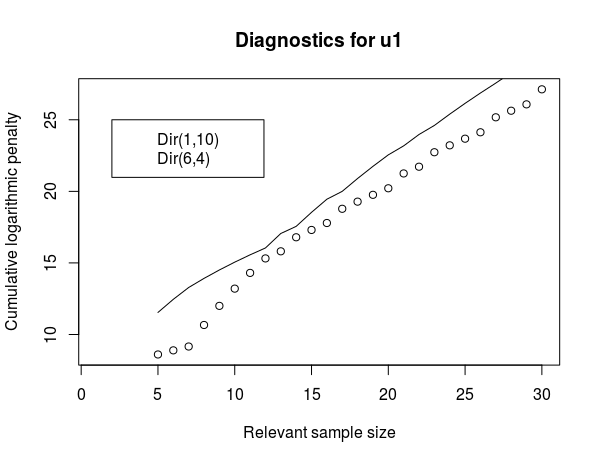
\includegraphics{Rplot.png}
%\end{figure}
%
%The reference prior is calculated by taking the total number of root to sink paths and dividing it by the number of variables at each floret. We compute the 


%\subsection{Food insecurity: summer meals example} 

%The data was obtained through

\section{Discussion}
 
\paragraph{Monitors}
The monitors can be used to detect misspecifications of structure or parameters. 

\paragraph{Missing data} The batch monitors are unable to detect 
Comparing the expert prior to the reference prior should in theory be invariant to the order in which the data is processed. However, in reality, the inferences may depend on the order of the data. 































































































































































































































































































































































































































































































































































































































































\end{document}
